%!TEX root =main.tex
\section{Application Highlights}\label{sec:applications}


In this section, we briefly review the  recent empirical successes of 
MARL driven by the methods introduced in the previous section. 
In the following, we focus on the three MARL settings reviewed in  \S\ref{sec:algorithms} and highlight  four representative and practical applications in each setting, as illustrated in Figure \ref{fig:app}. 

%\input{app_figure} 

\begin{figure*}[!t] 
	\centering
	\begin{tabular}{cccc}
		\hskip-10pt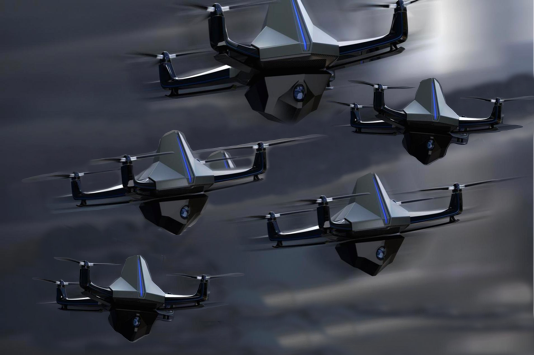
\includegraphics[width=0.24\textwidth]{Fig_3_app_uav}
		& 
		\hskip-5pt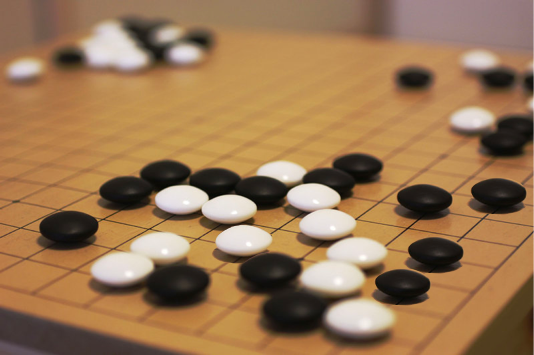
\includegraphics[width=0.24\textwidth]{Fig_3_app_go}
		&   
		  \hskip-5pt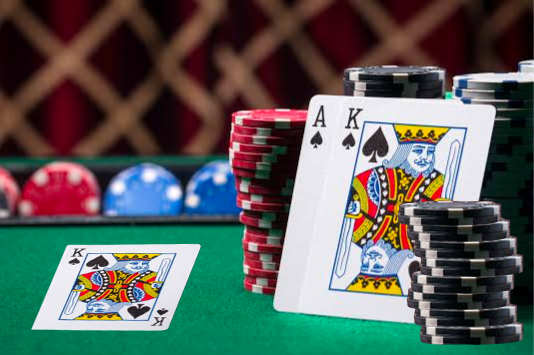
\includegraphics[width=0.24\textwidth]{Fig_3_app_poker}&   
		  \hskip-5pt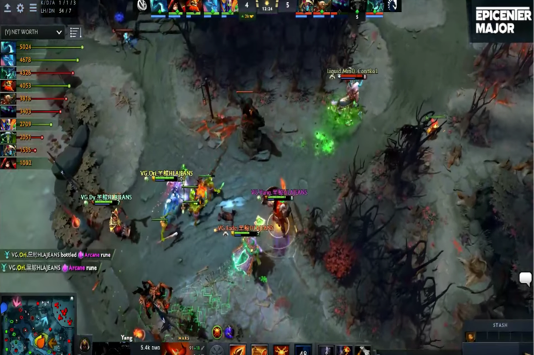
\includegraphics[width=0.24\textwidth]{Fig_3_app_dota}
%		  \\
%		\hskip-15pt(a) Centralized setting   & \hskip 6pt(b) Decentralized setting with networked agents & \hskip5pt (c) Fully decentralized setting	
\end{tabular}
	\caption{Four representative applications of recent successes of MARL: unmanned aerial vehicles, game of Go, Poker games, and team-battle video games. } 
	\label{fig:app} 
\end{figure*} 

\subsection{Cooperative Setting} \label{sec:application_coop}

\noindent{\bf Unmanned Aerial Vehicles}
\vspace{3pt}  

One  prominent application of MARL is the control of practical multi-agent systems, most of which are cooperative and decentralized. 
Examples of the scenarios include  robot team navigation \cite{corke2005networked}, smart grid operation \cite{dall2013distributed}, and control of mobile sensor networks \cite{cortes2004coverage}. Here we choose  unmanned aerial vehicles (UAVs) \cite{yang2018keeping,pham2018cooperative,tovzivcka2018application,shamsoshoara2019distributed,cui2019application,qie2019joint}, a recently surging application scenario of multi-agent autonomous systems, as one representative example. 
 Specifically, a team of  UAVs are deployed to accomplish a cooperation task, usually without the coordination of any central controller, i.e., in a decentralized fashion. Each UAV is  normally equipped with communication devices, so that they can exchange information with some of  their  teammates, provided that they are  inside its sensing and coverage range. As a consequence, this application naturally fits in the decentralized paradigm with networked agents we advocated in \S\ref{subsubsec:networked_paradigm}, which is also illustrated in Figure  \ref{fig:info_struc} (b). Due to the high-mobility of UAVs, the communication links among agents are indeed \emph{time-varying} and fragile, making (online)  cooperation extremely challenging. 
Various challenges thus arise in the  context of cooperative UAVs, some of which have recently been  addressed by MARL. 


In \cite{yang2018keeping}, the UAVs' optimal links discovery and selection problem is considered. Each UAV $u\in\cU$, where $\cU$ is the set of all UAVs, has the  capability to perceive the local available channels and  select a connected link over a common channel shared by another agent $v\in\cU$. Each UAV $u$ has its local set of channels $\cC_u$ with $\cC_u\bigcap \cC_v\neq \emptyset$ for any $u,v$, and a connected link between two adjacent UAVs is built if they announce their messages  on the same channel simultaneously.  Each UAV's local state is whether the previous  message has been successfully sent,  and its action is to choose a pair $(v,ch_u)$, with $v\in\cT_u$ and $ch_u\in \cC_u$, where $\cT_u$ is the set of teammates that agent $u$ can reach. The availability of local channels $ch_u\in \cC_u$ is modeled  as probabilistic, and the reward $\cR^u$ is calculated by the number of messages that are  successfully sent. Essentially, the algorithm in \cite{yang2018keeping} is based on independent Q-learning \cite{tan1993multi}, but with two heuristics to improve the tractability and convergence performance: by \emph{fractional slicing}, it  treats each dimension (fraction) of the action space independently, and  estimates the actual Q-value by the average of that for all fractions; by \emph{mutual sampling}, it shares both state-action pairs and a mutual Q-function parameter. 
  \cite{pham2018cooperative} addresses the problem of \emph{field coverage}, where the UAVs aim to provide a full coverage of an unknown field, while minimizing the overlapping sections among their field of views.  Modeled as a Markov team, the overall state $s$ is the concatenation of all local states $s_i$, which are defined as its $3$-D position coordinates  in the environment.  Each agent chooses to either head different directions, or go up and down, yielding $6$ possible actions.  A multi-agent Q-learning over the \emph{joint} action space is developed, with linear function approximation.  
In contrast, 
  \cite{shamsoshoara2019distributed} focuses  on spectrum sharing among a network of UAVs. Under a remote sensing task, the UAVs are categorized into two clusters: the relaying ones that provide relay services and  the other ones that gain  spectrum access for the remaining ones, which perform the sensing task. Such a problem can be modeled as a \emph{deterministic} MMDP, which can thus be solved by distributed Q-learning proposed in  \cite{lauer2000algorithm}, with optimality guaranteed.  Moreover, \cite{qie2019joint} considers the problem of \emph{simultaneous} target-assignment and path-planning for multiple UAVs. In particular, a team of UAVs $U_i\in\textbf{U}$, with each $U_i$'s position at time $t$ given by $(x_i^U(t),y_i^U(t))$, aim to cover all the targets $T_j\in\textbf{T}$ without collision with the threat  areas $D_i\in\textbf{D}$, as well as with other UAVs. For each $U_i$, a path  $P_i$ is planned  as $P_i=\{(x_i^U(0),y_i^U(0),\cdots,x_i^U(n),y_i^U(n))\}$, and the length of $P_i$ is denoted by $d_i$. Thus, the goal is to minimize $\sum_{i}d_i$ while the collision-free constraints are satisfied. 
  By penalizing the collision in the reward function, such a problem can be characterized as one with a mixed MARL setting that contains both cooperative and competitive agents. Hence, the MADDPG algorithm proposed in \cite{lowe2017multi} is adopted, with centralized-learning-decentralized-execution.  
  Two other tasks that can be tackled by MARL include resource allocation in UAV-enabled communication networks, using Q-learning based method \cite{cui2019application}, aerial surveillance and base defense in UAV fleet control, using policy optimization method in a purely centralized fashion \cite{tovzivcka2018application}.  
  

\vspace{6pt}
\noindent{\bf Learning to Communicate}
\vspace{3pt} 

Another application of cooperative MARL aims to foster  communication and coordination among a team of agents without explicit human supervision. 
Such a type of problems is usually formulated as a Dec-POMDP involving $N$ agents, which is similar to the Markov game introduced in Definition \ref{def:Markov_Game} except that
each agent cannot observe the state $s\in \cS$ and that each agent has the same reward function $\cR$. More specifically, we assume that 
  each agent $i \in \cN$ receives  observations from set $\cY^i$ via  a noisy observation channel $\cO^i \colon \cS \rightarrow \cP( \cY_i)$ such that agent $i$ observes a random variable $y^i \sim \cO^i (\cdot \given s)$ when the   environment is at state $s$.  Note that this model can be viewed as a POMDP when there is a central planner that collects the observations of each agent and decides the actions for each agent.
  Due to the noisy observation channels, 
  in such a model the agents need to communicate with each other so as to  better infer the underlying state and make decisions that maximize the expected return shared by all  agents. Let $\cN_t^{i} \subseteq \cN$  be the neighbors of agent $i$ at the $t$-th time step, that is, agent $i$ is able to receive a message $m_t^{j\rightarrow i}$ from any agent $j \in \cN_t^i$ at time $t$. Let $I_t^i $ denote  the information agent $i$ collects up to time $t$, which is defined as 
  \#\label{eq:information}
 I_t^i = \Bigl \{ \Big ( o_\ell ^i, \{ a_{\ell}^j \}_{j\in \cN } , \{  m_{\ell }^{j\rightarrow i} \}_{ j \in \cN_\ell^i }  \Bigr )  \colon \ell \in \{ 0, \ldots, t-1\} \Bigr \}  \bigcup \big \{ o_{t}^i,   \bigr \} ,
   \# 
   which contains its history collected in  previous time steps and the observation   received at time $t$. With the information $I_t^i$, agent $i$ takes an action $a_t^i \in \cA^i$ and also 
   broadcasts messages $m_t^{i\rightarrow j}$ to all agents $j$ with $i \in \cN_t^j$. That is,  the policy $\pi_t^i$ of agent $i$ is a mapping from $I^i_t$  to 
   a (random) action  $\tilde a_t^i =  (a_t^i, \{ m_{t}^{i\rightarrow j} \colon   i \in \cN_t^j \})$, i.e., $\tilde a_t^i \sim \pi_t^i ( \cdot \given I_t^i)$. 
   Notice that the 
   size of information  set  $I_t^i$ grows as $t$ grows. To handle the memory issue, it is common to first embed $I_t^i$ in a fixed latent space via recurrent neural network (RNN)  or Long Short-Term Memory (LSTM)  \cite{hochreiter1997long} and define the value  and policy functions on top of the embedded features. Moreover, most existing works in this line of research adopt the paradigm of centralized learning and utilize  techniques such as weight-sharing or attention mechanism \cite{vaswani2017attention} to increase computational efficiency.  With centralized learning, single-agent RL algorithms such as Q-learning and actor-critic are readily applicable.    
   
 In particular, 
    \cite{foerster2016learning} first proposes to tackle the problem of learning to communicate via deep Q-learning. They propose  to use two Q networks that govern taking action $a^i \in \cA$ and producing messages separately. Their training algorithm is an extension of the deep recurrent Q-learning (DRQN) \cite{hausknecht2015deep}, which combines RNN and deep Q-learning \cite{mnih2015human}. Following  \cite{foerster2016learning}, various works  \cite{jorge2016learning,sukhbaatar2016learning, havrylov2017emergence,  das2017learning,  peng2017multiagent, mordatch2018emergence, jiang2018learning, jiang2018graph, celikyilmaz2018deep, das2018tarmac, lazaridou2018emergence, cogswell2019emergence} have proposed a variety of neural network architectures to foster communication among agents. 
 These works combine single-agent RL methods with novel  developments in deep learning, and demonstrate their performance  via empirical studies. 
Among these works, \cite{das2017learning, havrylov2017emergence, mordatch2018emergence,lazaridou2018emergence,cogswell2019emergence} have reported the emergence of computational communication protocols among the agents when the RL algorithm is trained from scratch with text or image inputs.  We remark that the algorithms used in these works are more akin to single-agent RL due to centralized learning. For more details overviews of  multi-agent  communication, we  refer the interested readers to Section 6 of  \cite{oroojlooyjadid2019review} and Section 3 of \cite{hernandez2018multiagent}. 


\subsection{Competitive Setting} \label{sec:application_comp}

Regarding the competitive setting, in the following, we highlight the recent applications of MARL to \emph{the game of Go} and \emph{Texas hold'em  poker}, which are  archetypal instances of two-player perfect-information and partial-information extensive-form games, respectively.

\vspace{6pt}
\noindent{\bf The Game of Go}
\vspace{3pt} 


The game of Go is a board game played by two competing players, with the goal  of  surrounding more territory on the board than the opponent.  These two players have access to white or black stones respectively, and take turns placing their stones on a $19\times 19$ board, representing their territories. In each move, a player  can place a stone to any of the total $361$ positions on the board that is not already taken by a stone. Once placed on the board, the stones cannot be moved. But the stones will be removed from the board when completely surrounded by opposing stones. The game terminates when neither of the players is unwilling or unable to make a further move, and the winner is determined by counting the  area of the territory and the number of stones captured by the players.  

The game of Go can be viewed as a two-player zero-sum Markov game with deterministic state transitions, and the reward  only appears at the end of the game.  The state of this Markov game is the current configuration of the board and the reward is either one or minus one, representing either a win or a loss, respectively. Specifically,  we have $  r^1 (s)+ r^2(s)   =   0$ for any state $s\in \cS$, and   $r^1(s), r^2 (s) \in \{1, -1\}$ when $s$ is a terminating state, and $r^1 (s) = r^2 (s) = 0$ otherwise.  Let $V_{*}^i(s)$ denote the optimal value function of player $i \in \{1,2\}$.  Thus, in this case,  $[ 1+ V^{i}(s)]/2$ is  the probability of player $i\in \{1,2\}$  winning  the game when the current state is $s$ and both players follow the Nash equilibrium policies thereafter.  Moreover,
as this Markov game is turn-based, it is known that the Nash equilibrium policies of the two players are deterministic \cite{hansen2013strategy}. 
Furthermore,  since each configuration of the board can be constructed from a sequence of moves of the two players due to deterministic transitions, we can also view the game of Go as an extensive-form game with perfect information. 
This problem is notoriously challenging due to the gigantic state space. It is estimated in 
 \cite{allis1994searching}  that the size of state space  exceeds $10^{360}$, which forbids the usage of  any traditional reinforcement learning or searching algorithms.
 
A significant breakthrough has been made by the  \emph{AlphaGo}  introduced in  \cite{silver2016mastering},  which is the first computer Go program that defeats a human professional player on a full-sized board. AlphaGo integrates a variety of ideas from deep learning and reinforcement learning, and tackles the challenge of huge state space by representing the policy and value functions using deep convolutional neural networks (CNN) \cite{krizhevsky2012imagenet}. Specifically, both the policy and value networks are $13$-layer CNNs with the same architecture, and a board configuration is represented by $48$ features.  Thus, both the policy and value networks take  inputs of size 
 $19\times 19 \times 48$. 
These two networks are trained through  a novel combination of supervised learning from human expert data and reinforcement learning from Monte-Carlo tree search (MCTS) and self-play. Specifically, in the first stage, the policy network is trained by supervised learning to predict the actions made by the  human players, where the dataset consists of $30$ million positions from the KGS Go server. 
That is, for any state-action pair $(s,a)$ in the dataset, the action $a$ is treated as the response variable and the state $s$ is regarded as the covariate. The weights of  
  the policy network is trained via stochastic gradient ascent to maximize the likelihood function. 
  After initializing the policy network via supervised learning, 
 in the second stage of the pipeline, both the policy and value networks are trained via reinforcement learning and self-play. In particular, new data are generated by  games played between the current policy network and a random previous iteration of the policy network. Moreover, 
 the policy network is updated following policy gradient, 
 and the value network aims to find the value function associated with the policy network and is updated by minimizing the mean-squared prediction error. 
 Finally, when playing the game, the current iterates of the  policy and value networks are combined to produce an improved policy by lookahead search via MCTS. The actual action taken by AlphaGo is determined by such an MCTS policy. Moreover, to improve computational efficiency, AlphaGo uses an asynchronous and distributed version of MCTS to speed up   simulation. 
 
 Since the advent of AlphaGo, an improved version, known as  AlphaGo Zero, has been proposed in
  \cite{silver2017mastering}. 
  Compared with the vanilla AlphaGo, AlphaGo Zero does not use supervised learning to initialize the policy network. Instead, both the policy and value networks are trained from scratch solely via reinforcement learning and self-play. Besides, instead of having separate policy and value functions share the same network architecture, in AlphaGo Zero, these two networks are aggregated into a single neural network structure. Specifically, the policy and value functions  are represented by $(p(s), V(s)) = f_{\theta}(s)$, where $s \in \cS$ is the state which represents the current board, $f_{\theta}$ is a deep CNN with parameter $\theta$, $V(s)$ is a scalar that  corresponds to the value function, and  $p(s)$ is a vector which represents the policy, i.e., for each entry $a \in \cA$, $p_a(s) $ is the probability of taking action $a$ at state $s$. Thus, under such a network structure, the policy and value networks automatically share the same low-level representations of the states. Moreover, the parameter $\theta$ of network $f_{\theta}$ is trained via self-play and MCTS. Specifically, at each time-step $t$, based on the policy $p$ and value $V$ given by $f_{\theta_t}$, an MCTS policy $\pi_t$ can be obtained and a move is executed following policy $\pi_t(s_t)$. Such a simulation procedure continues  until the current  game terminates. Then the outcome of the $t$-th time-step, $z_t \in \{1, -1\}$,  is recorded, according to the perspective of the player at time-step $t$. Then the parameter $\theta$ is updated by following a stochastic gradient step on a loss function $\ell_t$, which is defined as 
  \$
  \ell_t(\theta) = [ z - V(s_t) ] ^2 - \pi_t^\top \log p(s_t) + c\cdot \|\theta \|_2^2 , \qquad \big ( p(\cdot) , V(\cdot)  \big) = f_{\theta} (\cdot) . 
  \$
  Thus, $\ell_t$ is the  sum of the mean-squared prediction error of the value function, cross-entropy loss between the policy network and the MCTS policy, and a weight-decay term for regularization. It is reported that 
  AlphaGo Zero has defeated the strongest versions of the previous AlphaGo and that it   also has demonstrated non-standard Go strategies  that had not been discovered  before. Finally, the techniques adopted in AlphaGo Zero has been generalized to other challenging board games. Specifically, 
\cite{silver2018general} proposes the AlphaZero program that is trained by self-play and reinforcement learning with zero human knowledge, and  achieves superhuman performance in the  games of chess, shogi, and Go. 

\vspace{6pt}
\noindent{\bf Texas Hold'em Poker}
\vspace{3pt} 


Another remarkable applicational achievement of MARL in the competitive setting focuses on developing artificial intelligence in the Texas hold'em poker, which is one of the most popular variations of the poker. Texas hold'em is usually played by a group of two or more players,
where each player is first dealt with two  \emph{private cards} face down. Then five \emph{community cards} are dealt face up in three  rounds. 
In each round. each player has four possible actions -- \emph{check}, \emph{call}, \emph{raise}, and \emph{fold}. 
After all the cards are dealt, each player who has not folded have seven cards in total, consisting of five community cards and two private cards. Each of these players  then  finds the best five-card poker hand out of all combinations of the seven cards. The player with the best hand is the winner and wins all the money that the players wager for that hand, which is also known as the \emph{pot}. Note that  each hand of Texas hold'em  terminates after three rounds, and the payoffs of the  player are only known after the hand ends. Also notice that each player is unaware of the private cards of the rest of the players. Thus, Texas hold'em is an instance of  multi-player extensive-form game  with incomplete information. 
The game is called \emph{heads-up} when there are only   two
players. When both the bet sizes and the amount of allowed raises are fixed, the game is called \emph{limit hold'em}. In the no-limit hold'em, however, each player may bet or raise any amount  up to all of the money the player has at the table, as long as  it exceeds the previous bet or raise. 

There has been quest for developing superhuman computer poker programs for over two decades \cite{billings2002challenge, rubin2011computer}. Various methods have been shown successful for simple variations of poker such as Kuhn  poker   \cite{kuhn1950simplified} and Leduc hold'em \cite{southey2005bayes}. However, the full-fledged Texas hold'em  is much more challenging and several breakthroughs have been achieved only recently.  The simplest version of Texas hold'em  is \emph{heads-up limit hold'em} (HULHE), which  has $3.9 \times 10^{14}$ information sets in total \cite{bowling2015heads}, where a player is required to take an action at each information set. \cite{bowling2015heads} has for the first time reported  solving HULHE to approximate Nash equilibrium  via  $\text{CFR}^{+}$ \cite{tammelin2014solving,tammelin2015solving}, a variant of counterfactual regret minimization \cite{zinkevich2008regret}. Subsequently, other methods such as Neural Fictitious Self-Play  \cite{heinrich2016deep}  and Monte-Carlo tree search with self-play \cite{heinrich2015smooth} have also been adopted to successfully solve HULHE. 

Despite these   breakthroughs, solving  \emph{heads-up no-limit hold'em} (HUNL) with artificial intelligence has remained open until recently, which has more than $6\times 10^{161}$ information sets, an astronomical number. Thus, in HUNL,  it is impossible (in today's computational power)  to traverse  all information sets, making it inviable to  apply  $\text{CFR}^{+}$ as in \cite{bowling2015heads}. Ground-breaking achievements have   recently been made by  \emph{DeepStack}  \cite{moravvcik2017deepstack} and \emph{Libratus}  \cite{brown2018superhuman}, two computer poker programs developed independently,  which defeat human professional poker players in HUNL for the first time. Both of these  programs adopt CFR as the backbone  of their algorithmic frameworks,  but  adopt different strategies for handling the gigantic size of the game. In particular, DeepStack applies  deep learning to learn good representations of the game and proposes \emph{deep counterfactual value networks} to integrate deep learning and CFR. Moreover, DeepStack adopts 
  limited depth lookahead planning to reduce the gigantic $6 \times 10^{161}$ information sets to no more than $10^{17}$ information sets, thus making it possible to enumerate all information sets.  
  In contrast, \emph{Libratus}   does not utilize any  deep learning techniques. Instead, it reduces the size of the game by computation of an abstraction of the game, which is possible since many of the information sets are very similar.  
  Moreover, it further reduces the complexity by using the  sub-game decomposition technique \cite{burch2014solving, moravcik2016refining, brown2017safe} for imperfect-information games and by constructing fine-grained abstractions  of the sub-games. When the abstractions are constructed, an improved version of the Monte-Carlo CFR \cite{lanctot2009monte, burch2012efficient,gibson2012generalized} is utilized to compute the policy. 
 Furthermore, very recently, based upon \emph{Libratus}, \cite{brown2019superhuman} has proposed  \emph{Pluribus}, a computer poker program  that has been shown to be stronger than top human professionals in   no-limit Texas hold'em poker with six players. The success of Pluribus is attributed to the  following  techniques that have appeared in the literature: abstraction and sub-game decomposition for large-scale imperfect-information games, Monte-Carlo CFR, self-play, and depth-limited search. 
 % In sum, CFR-based methods have demonstrated great promise in developing MARL systems for games with imperfect-information.  
    
    
    \vspace{6pt}
\noindent{\bf Other Applications}
\vspace{3pt} 


Furthermore, another popular testbed of MARL is the StarCraft II \cite{vinyals2017starcraft}, which is an immensely popular multi-player real-strategy computer  game.  This game can be formulated as a multi-agent Markov game with partial observation, where  each player  has only limited information of the game state. Designing reinforcement learning systems for StarCraft II is extremely challenging due to the needs to make  decisions  under uncertainty and incomplete information, to consider the optimal strategy in the long-run, and to design good reward functions that elicit learning. Since released, both the full-game and sub-game versions of  StarCraft II have gained tremendous research interest. 
A   breakthrough in this game was   achieved by    \emph{AlphaStar},   recently proposed in  \cite{vinyals2019grandmaster}, which has demonstrated superhuman performance in zero-sum two-player full-game StarCraft II.  Its reinforcement learning algorithm  combines   LSTM for the  parametrization of policy and value functions, asynchronous actor-critic  \cite{mnih2016asynchronous} for policy updates, and Neural Fictitious Self-play  \cite{heinrich2016deep} for equilibrium finding. 
%However, since discussion of   Markov games with partial observability is beyond the scope of this review, we refer the interested readers to \cite{vinyals2019grandmaster} for more  details of AlphaStar. 


 

\iffalse

\subsection{logic}
The applications that have driven the research on MARL:

1. cooperation setting: UAV control (decentralized control), learning to communicate 

2. zero-sum Markov games / (Extensive games): Go (complete information) and Poker (partial information) 

3. Non-cooperative Markov games-- computer games, NLP, and social science.


 
Change a title. ``Empirical success'' or ''applications''. \issue{Let's do not use empirical success, as for the networked settings, no empirical success yet. Just an application.}

{\color{red} idea: Introduce this task. Why this task is hard. Why that  RL method helps}



\remind{We may want to focus on some important applications that best-motivate the theory, or, some real-world applications that fit in the new theories developed.}


\fi 


 
\subsection{Mixed Settings}

Compared to the cooperative and competitive settings,  research on MARL  under the mixed setting is rather less explored. One  application in this setting is multi-player poker. As we have mentioned in \S\ref{sec:application_comp},  Pluribus introduced in  \cite{brown2019superhuman}  has  demonstrated superhuman performance in  six-player no-limit Texas hold'em.  In addition, as an extension of the problem of learning to communicate, introduced in 
\S\ref{sec:application_coop}, there is a line of research that aims to  apply MARL to tackle 
learning  social dilemmas, which is usually formulated as a multi-agent stochastic game with partial information. Thus, most of the algorithms proposed under these settings incorporate RNN or LSTM for learning representations of the histories experienced by the agent, and the performance  of  these algorithms are usually exhibited using experimental results;  see, e.g., \cite{leibo2017multi, lerer2017maintaining, hughes2018inequity}, and the references therein. 

 
Moreover, another example of the mixed setting is the case where the agents are divided into two opposing teams that play zero-sum games. The reward of a team is shared by each player within this team. Compared with two-player zero-sum games, this setting is more challenging in that both cooperation among teammates and competition against the opposing team  need to be taken into consideration. A   prominent testbed of this case is the \emph{Dota 2} video game, where  each of the two teams, each with five players, aims to conquer the base of the other team and defend its own base. Each player independently controls a powerful character known as the \emph{hero}, and only observes the state of the game via the video output on the screen. Thus, Dota 2 is a zero-sum Markov game  played by two teams, with each agent having imperfect information of the game. For this challenging problem, in 2018, \emph{OpenAI} has proposed the \emph{OpenAI Five} AI system \cite{OpenAI_dota}, which enjoys  superhuman performance and has  defeated human world champions in an e-sports game. The algorithmic framework integrates LSTM for learning good representations and proximal policy optimization \cite{schulman2017proximal} with self-play for policy learning. Moreover, to balance between effective coordination and communication cost, instead of having 
explicit communication channels among the teams, OpenAI Five utilizes reward shaping by having a hyperparameter, named ``team spirit'', to balance the relative importance between each hero's individual reward function  and the average of the team's reward function.   


%\remind{We will also mention a little on Deep MARL here.}
%
%\subsection{Deep MARL}

%Summarize the deep MARL algorithms for all the settings all together. 